\subsection{Radio Frequency Module Difference Test} % (fold)
\label{cha:radio_frequency_module_difference_test}
In tests using the RF Modules the difference in build quality and performance between the modules is a significant factor, and could be a source of error.
Consequently a test must be performed, which investigates these differences, so that the other test results can be validated.

\subsubsection*{Test setup}
To test all RF modules available to the group two Arduinos are used; one as receiver and the other as transmitter.
The RF modules are then switched in and out of breadboards connected to said Arduinos, so that both receiver and transmitter modules can be tested independently.
Furthermore a third Arduino is used to verify the results of each module.
The software on the Arduinos is the same as in the test in \myref[name]{cha:radio_frequency_module_reception_test}, i.e. a transmitting part which sends 100 unique packages and a receiving part which registers any package loss. 
Firstly modules is randomly tested to find a transmitter that shows very little to no package loss, thereafter every receiver is tested using the \enquote*{good} transmitter; with \enquote*{good} meaning a package loss very close to 0 \%, maximum 2 \%.
The same thing is done to test the transmitters, i.e. a \enquote*{good} receiver is used.
This approach is then repeated multiple times with different \enquote*{good} receivers and transmitters, to ensure a more fair test environment, with multiple combinations of modules.

\subsubsection*{Results}
The results have been plotted one bar chart, with the results of the different transmitters in the leftmost half, and the results of the different receivers in the rightmost.

\begin{figure}[H]
\centering
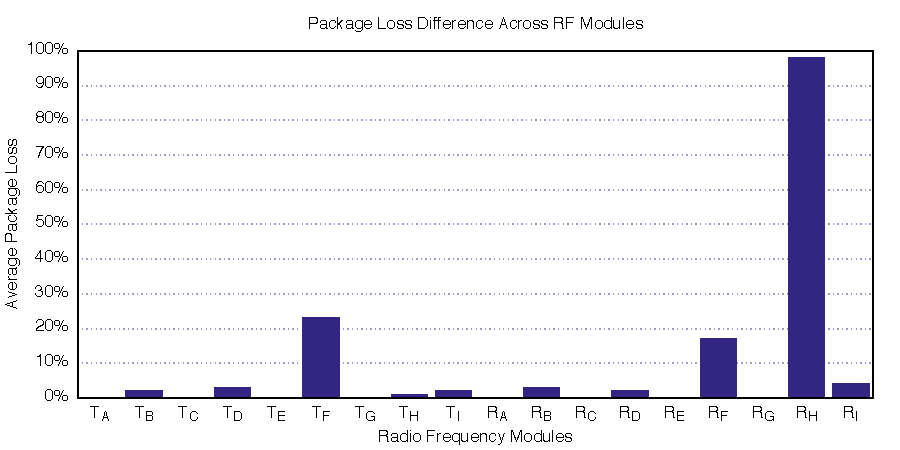
\includegraphics[width=\linewidth]{Figures/Graphs/diff_graph.pdf}
\centering
\caption{The average package loss inflicted by the radio frequency modules.\\ \textsf{T}\textsubscript{\textit{device}} denotes transmitters and \textsf{R}\textsubscript{\textit{device}} denotes receivers.}    
\label{fig:trans_diff}
\vspace{-20pt}        
\end{figure} 

\subsubsection*{Conclusion}
When looking at the results of this test, it is clear that some of the modules were significantly worse at respectively transmitting and receiving data.
Transmitter \textsf{T\textsubscript{F}} inflicted an average package loss over 20 \%, and receiver \textsf{R\textsubscript{H}} failed to receive more than 2 \% of the packages on average.
Moreover receiver \textsf{R\textsubscript{F}} had an average package loss just below 20 \%.
However to ensure validity of other tests using the RF Modules, the group will exclude the three faulty modules (transmitter \textsf{T\textsubscript{F}}, receiver \textsf{R\textsubscript{H}}, and receiver \textsf{R\textsubscript{F}}) from these tests.
% chapter radio_frequency_module_difference_test (end) 
